\chapter{Autoconfiguración de direcciones en redes descentralizadas}
%-----------------------------------
%   AUTOCONFIGURACIÓN DE DIRECCIONES
%-----------------------------------
\label{ch:autoconfiguracion_de_direcciones_en_redes_descentralizadas}

Antes de que cualquier dispositivo pueda comunicarse a través de una red,
necesita tener asignada una dirección. Una dirección es un número que identifica
a un nodo dentro de una red. Cuando un paquete va destinado a una dirección,
ésta tiene que estar asignada a un solo dispositivo, de otro modo, no habría
manera de saber a cuál va dirigido.

La configuración manual consiste en que una persona configure la dirección.
Sin embargo, al requerir la intervención humana, es un proceso muy lento.
Este método resulta especialmente inconveniente cuando se trata de dispositivos
móviles, ya que estos dispositivos están diseñados para conectarse y
desconectarse con frecuencia en diferentes redes inalámbricas.

En las redes de infraestructura fija, la configuración de los nodos es
realizada, por lo general, por un servidor \textit{Dynamic Host Configuration
Protocol} (DHCP), que conoce las direcciones que están siendo ocupadas por todos
los nodos. Cuando un nodo se quiere unir a la red, contacta al servidor DHCP para
solicitarle una dirección IP, y éste le ofrece una dirección disponible
\cite{Kurose2013}. Este método es efectivo en una red de infraestructura fija,
ya que todos los nodos pueden contactar a través del enlace local al servidor
DHCP. En un MANET, la única manera que tendrían la mayoría de los nodos para
contactar a un servidor DHCP sería a través de nodos intermedios, que tienen la
libertad de moverse sin ninguna restricción. Por esta razón, no es factible que
un servidor DHCP se encargue de la configuración de direcciones en una red
descentralizada.

En las MANETs, los protocolos de autoconfiguración de direcciones son
responsables de asignar la dirección a cada nodo, garantizando su unicidad. A
continuación, se presentan los tipos de protocolos de autoconfiguración de
direcciones que se han desarrollado, así como algunos de los protocolos más
representativos de cada uno.

En este capítulo, se presenta el protocolo IPv6, que es el que rige el
funcionamiento de la retransmisión de paquetes, y especifica el formato de las
direcciones. Posteriormente, se presentan diferentes protocolos que se han
propuesto para la configuración autmática de direcciones para MANETs.

\section{Protocolo IPv6}
%-----------------------------------
%   PROTOCOLO IPV6
%-----------------------------------
\label{sec:protocolo_ipv6}

El protocolo \textit{Internet Protocol} (IP)\footnote{Protocolo de Internet.}
forma parte de la capa de red, y es el que rige la retransmisión de paquetes
a través de los enrutadores para que lleguen a su destino. Este protocolo
especifica en cada paquete cuál es el nodo de origen y cuál es el nodo de
destino (también llamado datagrama). Cada nodo se identifica de manera única
mediante un número llamado \keyword{dirección IP}. Cuando un enrutador obtiene
la dirección de destino de un paquete, consulta la mejor ruta y lo retransmite
al siguiente \cite{Kurose2013}.

La versión IPv4 fue desarrollada a principios de la década de 1970, y ha tenido
la hegemonía en la Internet durante más de 30 años. Pero desde hace más de dos
década se ha hecho cada vez más evidente su obsolescencia. Su limitación más
importante es que la cantidad de direcciones que ofrece ya se ha visto rebasada
por la cantidad de usuarios de Internet en el mundo \cite{Hagen2006}.

En 1993, se comenzó a desarrollar la versión IPv6, considerando las debilidades
de la versión anterior. La más importante mejora se encuentra en el tamaño de
las direcciones, ya que ofrece un espacio de direcciones más que suficiente
para identificar a todos los dispositivos del mundo, a diferencia de su
predecesor \cite{Hagen2006}.

\subsection{Datagrama IPv6}
%-----------------------------------
%   DATAGRAMA IPV6
%-----------------------------------
\label{subsec:datagrama_ipv6}

En la capa de red, la unidad de datos del protocolo se conoce como datagrama.
En el protocolo IPv6, un datagrama tiene una cabecera que contiene información
que los enrutadores analizan para realizar el enrutmaiento.En la figura
\ref{fig:formato_datagrama_ipv6_general} se muestra el formato de un datagrama
IPv6 \cite{Hagen2006}.

\begin{figure}[th]
\centering
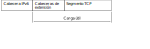
\includegraphics{formato_datagrama_ipv6_general}
\decoRule
\caption[Datagrama IPv6]{Formato de un datagrama IPv6.}
\label{fig:formato_datagrama_ipv6_general}
\end{figure}

El formato de la cabecera IPv6 se muestra en la figura
\ref{fig:formato_cabecera_ipv6}, y se forma por los siguientes campos
\cite{RFC2460}:

\begin{figure}[th]
\centering
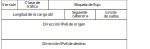
\includegraphics{formato_cabecera_ipv6}
\decoRule
\caption[Cabecera IPv6]{Formato de la cabecera IPv6.}
\label{fig:formato_cabecera_ipv6}
\end{figure}

\keyword{Versión (4 bits)} -- Versión del protocolo IP.

\keyword{Clase de tráfico (1 byte)} -- Prioridad asignada al datagrama.

\keyword{Etiqueta de flujo (20 bits)} -- Identificar una secuencia de
datagramas.

\keyword{Longitud de carga útil (2 bytes)} -- Número de bytes de la carga útil.

\keyword{Siguiente cabecera (1 byte)} -- Identifica el tipo de cabecera que
sigue después de la cabecera IPv6.

\keyword{Límite de saltos (1 byte)} -- Número de veces que se ha
retransmitido el datagrama. Es decrementado por cada enrutador que lo
retransmite. Si llega a cero, se descarta el datagrama.

\keyword{Dirección IPv6 de origen (16 bytes)} -- Dirección IPv6 del dispositivo
que originó el datagrama.

\keyword{Dirección IPv6 de destino (16 bytes)} -- Dirección IPv6 del dispositivo
al que va dirigido el datagrama.

\subsection{Direccionamiento IPv6}
%-----------------------------------
%   DIRECCIONAMIENTO IPV6
%-----------------------------------
\label{subsec:direccionamiento_ipv6}

Una dirección IP es un número que identifica de manera única cada interfaz de
red de un dispositivo. Comúnmente se asocia la dirección IP con el dispositivo.
Sin embargo, si un dispositivo tiene más de una interfaz, puede tener más de una
dirección IP. Incluso una sola interfaz puede tener asignadas varias
direcciones.

En la dirección se encuentra la información de la red a la que está conectada la
interfaz, así como el identificador único de la interfaz dentro de esa red. Con
esta estructura jerárquica, cuando se enruta un paquete hacia su destino, el
primer objetivo es que el paquete llegue a la red correspondiente. Una vez que
el paquete llega a la red, se hace un enrutamiento local para que llegue al
nodo correspondiente \cite{Kurose2013}.

En el protocolo IPv6, las direcciones tienen una longitud de 128 bits. Con un
espacio de direcciones de tamaño $2^128$, se cuenta con suficientes para asignar
una (o más si fuera necesario) a cada dispositivo que existe. Esta fue la
principal motivación de la creación del protocolo IPv6, aunque incluye muchas
otras mejoras respecto a IPv4 \cite{Hagen2006}.

Una dirección IPv6 se divide en ocho bloques de 16 bits, que se representan en
notación hexadecimal y se separan con \code{:}. Cuando hay una secuencia de
bloques que contiene únicamente ceros, se puede comprimir usando \code{::}. Por
ejemplo:

\noindent\code{2001:DB8:0:0:202:B3FF:FE1E:8329}\\
\code{2001:DB8::202:B3FF:FE1E:8329}

La notación de prefijo se usa para representar un bloque del espacio de
direcciones. Por ejemplo:

\noindent\code{2E78:DA53:1200::/40}

Este prefijo representa todas las direcciones posibles que comienzan con
los primero 40 bits de la dirección \code{2E78:DA53:1200::}. Generalmente, el
prefijo corresponde al identificador de la red; sin embargo, hay prefijos que
tienen significados especiales \cite{Hagen2006}.

El protocolo IPv6 define tres tipos de direcciones \cite{CiscoIpv62011}:

\keyword{\textit{Unicast}} -- Identifica una única interfaz en un nodo. Los
paquetes que se envían a una dirección \textit{unicast} son entregados
solamente a dicha interfaz.

\keyword{\textit{Anycast}} -- Una dirección \textit{anycast} puede ser asignada
a interfaces de diferentes nodos. Los paquetes dirigidos a una dirección de este
tipo sólo llegan a la interfaz más cercana que tenga asignada la dirección,
según los protocolos de enrutamiento.

\keyword{\textit{Multicast}} -- Es un identificador para un conjunto de
interfaces, que generalmente pertenecen a nodos distintos. Cuando un paquete
se envía a una dirección \textit{multicast}, éste llega a todas las interfaces
que pertenecen al gurpo.


\section{Autoconfiguración de direcciones con estado}
%-----------------------------------
%   AUTOCONFIGURACIÓN DE DIRECCIONES CON ESTADO
%-----------------------------------
\label{sec:autoconfiguracion_de_direcciones_con_estado}

El protocolo DHCP es el ejemplo más claro de este tipo de protocolos. Se dice
que es con estado debido a que mantiene en todo momento el registro de todos los
nodos que formar parte de la red y la dirección de cada uno. A pesar de que este
enfoque tiene una aplicación limitada en las MANETs, se han desarrollado
métodos de configuración con estado para este tipo de redes. Estos se basan,
principalmente, en la distribución y administración de las direcciones entre un
grupo de nodos de manera descentralizada \cite{Grajzer2019}.

El protocolo MANETconf \cite{Nesargi2002} es uno de los más representativos de
esta categoría. En este protocolo, todos los nodos tienen el registro de todas
las direcciones que se han asignado en la red. Cuando un nuevo nodo, denominado
\textit{solicitante}, quiere unirse a una red, contacta a un nodo que tenga a su
alcance, llamado \textit{iniciador}. En iniciador envía una solicitud al resto
de los nodos para saber si una dirección está disponible. Cuando recibe una
respuesta positiva de todos los demás nodos, le puede asignar la dirección al
solicitante. Después, el iniciador envía la notificación de que la dirección ya
se encuentra en uso al resto de los nodos. Este protocolo tiene varias
desventajas, como la necesidad de que todos los nodos cuenten con espacio para
almacenar todas las direcciones en uso, así como un alto uso de los recursos de
la red, ya que se tiene que inundar con solicitudes y notificaciones cada vez
que se une un nuevo nodo.

Un método para reducir el problema de la sobrecarga de la red que presenta el
protocolo MANETconf, es propuesto por Munjal \textit{et al.} \cite{Munjal2014},
en el que el iniciador no espera confirmaciones de todos los demás nodos cuando
envía una solicitud. Cuando un nodo recibe la respuesta del iniciador, éste
responde únicamente si tiene que avisarle que la dirección se encuentra en uso.
Esto reduce significativamente el uso de los recursos de la red, sin embargo,
aún se debe inundar con una solicitud cuando un iniciador necesita asignar una
dirección. Además, como en el protocolo MANETconf, los nodos deben tener la
lista de todas las direcciones en uso.

El protocolo \textit{Mobile Agents based Address Auto-Configuration}
(MAAC)\footnote{Autoconfiguración de direcciones basada en agentes móviles.} fue
propuesto por Korichi \textit{et al.} \cite{Korichi2018}. En este protocolo,
los nodos de la red se organizan jerárquicamente en grupos, y cada grupo es
administrado por un agente móvil alojado en uno de los nodos. Este sistema
móvil multi-agente forma servidor virtual como sustituto de un servidor DHCP.
Cuando un nodo se quiere unir a la red, envía una solicitud de dirección a los
nodos cercanos, y cada uno reenvía la solicitud al agente que lo configuró. Si
un agente recibe la solicitud, responde con una propuesta de de dirección. El
nodo que originó la solicitud úicamente considera la propuesta del agente que
está a menos saltos de distancia.

Este tipo de protocolos tienen el inconveniente de requerir el mantenimiento de
las tablas con las direcciones de todos los nodos de la red, cuyo tamaño
incrementa confome se incorporan nuevos nodos. Esto hace que, mientras más
grande se hace la red, se necesitan más recursos, tanto computacionales como de
comunicación.

\section{Autoconfiguración de direcciones sin estado}
%-----------------------------------
%   AUTOCONFIGURACIÓN DE DIRECCIONES SIN ESTADO
%-----------------------------------
\label{sec:autoconfiguracion_de_direcciones_sin_estado}

En la configuración automática sin estado, cada nodo se asigna su propia
dirección, y no necesita mantener información de las direcciones de todos los
demás nodos. En general, para que un nuevo nodo pueda obtener una dirección, se
lleva a cabo un proceso llamado \textit{Duplicate Address Detection}
(DAD)\footnote{Detección de direcciones duplicadas.}. Cuando un nodo quiere
unirse a la red, envía una consulta con una dirección tentativa a todos los
demás nodos. Si alguno ya tiene asignada esta dirección, le envía una
notificación al nodo nuevo, y este repite este proceso. Si no recibe ninguna
respuesta dentro de un intervalo de tiempo, asume que la dirección está
disponible y puede usarla \cite{Grajzer2019}.

El protocolo \textit{Address Reservation and Optimistic Duplicated address
detection} (AROD)\footnote{Resesrvación de direcciones y detección optimista de
direcciones suplicadas.} propuesto por Kim \textit{et al.} \cite{Kim2007}
funciona mediante la reservación de direcciones, lo que reduce el tiempo de
configuración y el uso del ancho de banda de la red. Este protocolo define tres
tipos de nodos:
\begin{enumerate*}[label=\arabic*)]
  \item un nodo que tiene reservada una dirección además de su propia dirección;
  \item un nodo que no tiene ninguna dirección reservada;
  \item un nuevo nodo
\end{enumerate*}.
Cuando un nuevo nodo quiere entrar a la red, selecciona uno de sus vecinos
como agente, que se encarga de asignarle una dirección. Si el agente es de tipo
1, le asigna la dirección reservada inmediatamente. Si el agente es de tipo 2,
le solicita la dirección reservada a otro nodo de tipo 1. Esta operación
resulta más eficiente que el procedimiento DAD, ya que requiere un único
mensaje \textit{broadcast}.

Después de la configuración de un nuevo nodo, el agente selecciona dos
direcciones al azar, y realiza la operación DAD para cada una. Si ambas
direcciones son únicas, el agente reserva una y el nuevo nodo reserva otra, y
ambos nodos son de tipo 1. Si una dirección está ocupada, al agente reserva la
dirección libre, y el nuevo nodo es de tipo 2. Si ninguna dirección está
disponible, tanto el agente como el nuevo nodo son de tipo 2. Este protocolo
requiere baja demanda de comunicación de la red, además de que garantiza que
las direcciones son únicas.

En \cite{Munjal2015}, Mujal presenta el protocol \textit{Scalable
Hierarchical Distributive Auto-Configuration Protocol} (
SHDACP-IPv6)\footnote{Protocolo de autoconfiguración distributiva jerárquica
escalable.}.
En este protocolo, las direcciones IPv6 se componen de cinco campos, como se
ilustra en la figura \ref{fig:formato_direccion_shdacp}: prefijo (7 bits),
identificador global (41 bits), identificador de partición (16 bits),
identificador de grupo (48 bits) e identificador de red (16 bits).

\begin{figure}[th]
\centering
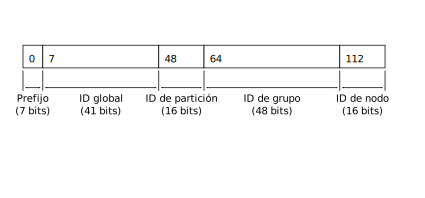
\includegraphics{formato_direccion_shdacp}
\decoRule
\caption[Formato de las direcciones del protocolo SHDACP-IPv6]{Formato de las
direcciones del protocolo SHDACP-IPv6\protect\footnotemark.}
\label{fig:formato_direccion_shdacp}
\end{figure}

\footnotetext{Adaptación del esquema presentado por Mujal \cite{Munjal2015}.}

Cuando un nodo, denominado \textit{solicitante}, se quiere unir a una red,
transmite un mensaje \textit{Neighbor\_Query}, esperando recibir como respuesta
al menos un mensaje \textit{Neighbor\_Reply} de otro nodo ya configurado. Si no
recibe respuesta, repite el proceso. Después de cierta cantidad de intentos, si
no recibe respuesta, el solicitante asume que es el primer nodo de la red, y se
autoconfigura como \textit{Cluster Head} (CH), o cabeza de grupo, con un número
de partición aleatorio, un número de grupo aleatorio y el identificador de nodo
1. Cuando otro nodo se quiere unir a la red, el CH recibe una solicitud de
éste, y le asigna un identificador de nodo secuencialmente. Si un nuevo nodo se
encuentra a más de cierto número de saltos de distancia de todos los CHs, se
autoconfigura como un nuevo CH.

Este protocolo también cuenta con mecanismos para lidiar con particiones de la
red, causadas por el movimiento impredecible de los nodos, así como para
combinar dos o más particiones. Sin embargo, no garantiza que no existan
direcciones repetidas, pero gracias al amplio espacio de direcciones que ofrece
el protocolo IPv6, la probabilidad de que esto ocurra es casi nula.

El protocolo IPv6 especifica un procedimiento cuyo propósito es ayudar a
llevar a cabo la autoconfiguración de direcciones sin estado, llamado
\textit{Neighbor Discovery} (ND)\footnote{Descubrimiento de vecinos.}. Cuando un
nodo quiere obtener una dirección, envía un mensaje \textit{Neighbor Solicitation}
(NS), o solicitud de vecino, a sus vecinos directos. Si alguno ya tiene asignada
la dirección, responde con un mensaje \textit{Neighbor Advertisement} (NA), o
anuncio de vecino. Sin embargo, este procedimiento no se puede aplicar en una
MANET, ya que funciona únicamente dentro del alcance del enlace local.

Grajzer \textit{et al.} \cite{Grajzer2019} proponen ND++, una extensión del
estándar ND que agrega dos tipos de mensajes: \textit{multihop Neighbor
Solicitation} (mNS), o solicitud de vecino multi-salto, y \textit{multihop
Neighbor Advertisement} (mNA), o anuncio de vecino multi-salto. Cuando un nodo
realiza el procedimiento DAD y determina que su dirección no está en uso por
sus vecinos directos, ejecuta el procedimiento DAD++, en el que inunda la red
con un mensaje mNS, esperando como respuesta un mensaje mDA. ND++ usa una
técnica de optimización de inundación que sólo requiere conocer los vecinos que
se encuentran hasta dos saltos de distancia de cada nodo, limitando el
intercambio de mensajes de control necesarios únicamente al enlace local.
